\documentclass[pt,oneside,onehalfspacing,msc]{risethesis}

\usepackage{babel}
\usepackage[utf8]{inputenc}
\usepackage[linesnumbered,vlined,ruled,boxed,commentsnumbered]{algorithm2e}
\usepackage{algpseudocode}
\usepackage{bm} % Allows bold greek letters for representing vectors

% math equations
\usepackage{amsmath,amssymb,amsfonts}
\usepackage{commath}
\usepackage{float}

\usepackage[flushleft]{threeparttable}

\usepackage{colortbl}
\usepackage{color}
\usepackage[table]{xcolor}
\usepackage{microtype}
\usepackage{bibentry}
\usepackage{subfig}
\usepackage{multirow}
\usepackage{rotating}
\usepackage{booktabs}
\usepackage{pdfpages}
\usepackage{lipsum}
\usepackage{scalefnt}

% Configurando layout para mostrar codigos Java
\usepackage{listings}
\newcommand{\estiloJava}{
\lstset{
    language=Java,
    basicstyle=\ttfamily\small,
    keywordstyle=\color{jpurple}\bfseries,
    stringstyle=\color{red},
    commentstyle=\color{verde},
    morecomment=[s][\color{blue}]{/**}{*/},
    extendedchars=true,
    showspaces=false,
    showstringspaces=false,
    numbers=left,
    numberstyle=\tiny,
    breaklines=true,
    backgroundcolor=\color{cyan!10},
    breakautoindent=true,
    captionpos=b,
    xleftmargin=0pt,
    tabsize=2
}}

\let\counterwithout\relax
\let\counterwithin\relax
\usepackage{chngcntr}

\usepackage[tocflat,toctextentriesindented]{tocstyle}
\deactivatetocstyle[lof]
\deactivatetocstyle[lot]
\deactivatetocstyle[loa]

\usetocstyle{allwithdot}
\settocfeature[toc][0]{entryhook}{\bfseries\uppercase}
\settocfeature[toc][1]{entryhook}{\uppercase}
\settocfeature[toc][2]{entryhook}{\bfseries}
\settocfeature[toc][3]{entryhook}{\itshape}

\settocfeature{spaceafternumber}{3em}
\makeatletter
\renewcommand*\l@figure{\@dottedtocline{1}{1.5em}{5.9em}}
\renewcommand*\l@table{\@dottedtocline{1}{1.5em}{5em}}
\makeatother

\usepackage{titlesec}
\titleformat{\section}{\normalfont\large}{\thesection}{1em}{\MakeUppercase}
\titleformat{\subsection}{\normalfont\large}{\bfseries\thesubsection}{1em}{\bfseries}
\titleformat{\subsubsection}{\normalfont\large}{\itshape\thesubsubsection}{1em}{\itshape}

\newcommand{\fref}[1]{\figurename \ref{#1}}
\newcommand{\tref}[1]{\tablename \ref{#1}}
\newcommand{\sref}[1]{\sectionname \ref{#1}}
\newcommand{\eref}[1]{\equationame \ref{#1}}
\newcommand{\aref}[1]{\algname \ref{#1}}
\newcommand{\chref}[1]{\chaptername \ref{#1}}

% \captionsetup[table]{position=top,justification=centering,width=.85\textwidth,font=small, labelsep=newline}
% \captionsetup[lstlisting]{position=top,justification=centering,width=.85\textwidth,labelfont=bf,font=small}
% \captionsetup[figure]{position=bottom,justification=centering,width=.85\textwidth,labelfont=bf,font=small}

% -----------------------------------------------------------
% settings for the list of acronyms
% begin
% -----------------------------------------------------------
% \usepackage[noredefwarn,acronym]{glossaries} %GLOSSÁRIO

\newcolumntype{L}[1]{>{\raggedright\let\newline\\\arraybackslash\hspace{0pt}}m{#1}}
\newcolumntype{C}[1]{>{\centering\let\newline\\\arraybackslash\hspace{0pt}}m{#1}}
\newcolumntype{R}[1]{>{\raggedleft\let\newline\\\arraybackslash\hspace{0pt}}m{#1}}

\newglossarystyle{modsuper}{%
  \setglossarystyle{super}%
  \renewcommand{\glsgroupskip}{}

% put the glossary in a longtable environment:
 \renewenvironment{theglossary}%
  {
    \begin{longtable}
        {L{0.3\textwidth}L{0.7\textwidth}}}%
    {\end{longtable}
    \addtocounter{table}{-1}
  }
}

% -----------------------------------------------------------
% settings for the list of acronyms
% end
% -----------------------------------------------------------

%% Change the following pdf author attribute name to your name.
\usepackage[linkcolor=black,
            citecolor=blue,
            urlcolor=black,
            colorlinks,
            pdfpagelabels,
            pdftitle={M.Sc. Dissertation - Samuel Bristot loli},
            pdfauthor={Samuel Bristot loli}]{hyperref}

\definecolor{jpurple}{rgb}{0.5,0,0.35}

\address{Recife}

\universitypt{Universidade Federal de Pernambuco}
\universityen{Federal University of Pernambuco}

\departmentpt{Centro de Informática}
\departmenten{Center of Informatics}

\programpt{Pós-graduação em Ciência da Computação}
\programen{Graduate in Computer Science}

\majorfieldpt{Ciência da Computação}
\majorfielden{Computer Science}

\concentrationareapt{Inteligência Computational}
\concentrationareaen{Computational Intelligence}

\title{Title}

\date{2019}

\author{Samuel Bristot Loli}
\adviser{Leopoldo Teixeira}

% Macros (defines your own macros here, if needed)
\def\x{\checkmark}

\setlength{\headheight}{16pt} %Solucao para o Erro:Package Fancyhdr Warning: \headheight is too small (12.0pt)

% ----------------------------------------------------------
% import list of acronyms and symbols
% ----------------------------------------------------------
\newacronym{som}{SOM}{Self-Organizing Map}
\newacronym{svhn}{SVHN}{Street View House Numbers}
\newacronym{cifar10}{CIFAR10}{Canadian Institute For Advanced Research}

\newglossaryentry{updatestep}{
  name = $\Delta$,
  description = Gradient
}

\makenoidxglossaries

\renewcommand*{\glsseeformat}[3][\seename]{\textit{#1}
\glsseelist{#2}}

\renewcommand*{\glspostdescription}{} % remove trailing dot
\renewcommand{\glsnamefont}[1]{\textbf{#1}}
\renewcommand{\glossarypreamble}{\thispagestyle{empty}}
% ----------------------------------------------------------
% ----------------------------------------------------------

% ----------------------------------------------------------
% continuous couting for tables and figures
% ----------------------------------------------------------
\counterwithout{figure}{chapter}
\counterwithout{table}{chapter}
% ----------------------------------------------------------
% ----------------------------------------------------------

\renewcommand{\listalgorithmcfname}{\MakeUppercase{\bfseries\Large{\listalgorithmsname}}}
\renewcommand{\algorithmcfname}{\algname}

\begin{document}

 \frontmatter

 \frontpage

 \presentationpage

 \catalog

 \banca

 \begin{dedicatory}
I dedicate this dissertation to all my family.
\end{dedicatory}


 \acknowledgements


 % \begin{epigraph}[]{Arthur Ashe}
``Start where you are. Use what you have. Do what you can."
\end{epigraph}


 \abstract
Abstract

\begin{keywords}
X. Y. Z.
\end{keywords}


 \resumo
Resumo.
\begin{keywords}
X. Y. Z.
\end{keywords}


 {
 \let\oldnumberline\numberline
 \newcommand{\fignumberline}[1]{\figurename~#1~\enspace--~\enspace}
 \renewcommand{\numberline}{\fignumberline}
 \listoffigures
 }

 {
 \let\oldnumberline\numberline
 \newcommand{\tabnumberline}[1]{\tablename~#1~\enspace--~\enspace}
 \renewcommand{\numberline}{\tabnumberline}
 \listoftables
 }

 \listofacronyms

 \listofsymbols

 {
 \let\oldnumberline\numberline
 \newcommand{\algnumberline}[1]{\algname~#1~\enspace--~\enspace}
 \renewcommand{\numberline}{\algnumberline}
 \listofalgorithms
  }

% Summary (tables of contents)
\tableofcontents

\mainmatter

 \chapter{Introdução}
\label{chap:intro}

\gls{som} \citep{som}.

teste \citep{Chen:2014:DPA:2568225.2568259}

\begin{figure}[H]
	\centering
	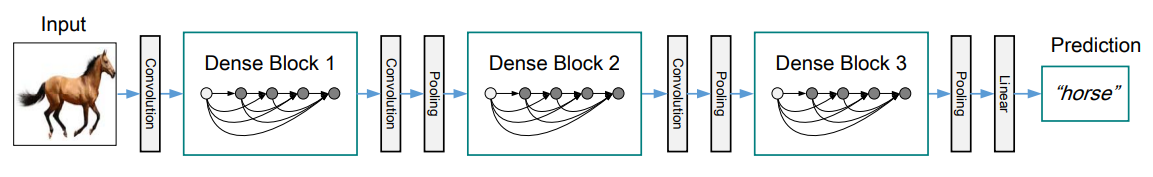
\includegraphics[width=\linewidth]{figures/densenet}
	\caption{\textmd{DenseNet architecture}}
	\label{fig:densenet-model}
\end{figure}


\begin{equation}
\label{eq:ce}
CE(C, C^\prime) =  \frac{|U| - D_{max}}{|U|},
\end{equation}


\begin{table}[ht]
\small
\centering
\begin{threeparttable}
\renewcommand{\arraystretch}{1.3}
\caption{Specifications of the Deep Learning Benchmark Image Datasets}
\label{tab:deep-datasets}
\centering
\begin{tabular}{c|ccc}
\hline
\bfseries  Datasets & \bfseries Resolution & \bfseries Channels & \bfseries Classes\\
\hline
\gls{cifar10} & 32 x 32 & 3 & 10 \\
\gls{svhn} & 32 x 32 & 3 & 10 \\
MNIST & 28 x 28 & 1 & 10 \\
FashionMNIST & 28 x 28 & 1 & 10 \\
\hline
\end{tabular}
\end{threeparttable}
\end{table}


\begin{algorithm}[!ht]
Initialize parameters;

\For{epoch $\gets$ 0 \textit{\textbf{to}} $epoch_{max}$}
{
	Choose a random input pattern $\boldsymbol{x}$;

	\eIf{\text{condition}}
    {
    	Run X;

    } {
    	Run Y.;
    }
}

\caption{Algorithm}
\label{alg:algorithm}
\end{algorithm}


\chapter{Catálogo - ORM Bad Smell}
\label{chap:badsmell}

\section{Dados em excesso}
\label{dados_excesso}
Segundo \cite{hibernate_543}, trazer dados em excesso do banco de dados para a aplicação pode ser considerado o problema de desempenho número um na maioria das aplicações que utilizam JPA. A seguir serão listados possíveis \textit{bad smells} relacionados a este problema.

\subsection{\textit{EAGER} como estratégia de busca nas associações a nível de classe}
\label{subsection:EAGER_ESTATICO}
Uma das causas de excesso de dados em frameworks ORM é a utilização indevida da estratégia de busca do tipo \textit{EAGER} (ansioso). Esta estratégia de busca é utilizada para carregar previamente as informações do banco de dados de um objeto relacionado.
O mapeamento pode ser realizado de forma estática, utilizando uma anotação a nível de classe referenciando o atributo que representa outro objeto, de forma a sempre carregar o objeto relacionado.  Por exemplo: objeto A possui um atributo relacionado ao objeto B. Utilizando \textit{EAGER}, sempre que qualquer atributos do objeto A for carregado, o objeto B também será, independente se alguma informação do objeto B será utilizada. \citep{bauer2005hibernate}

%TODO: Adicionar exemplo com imagem do código

Segundo a documentação oficial, a utilização da estratégia de busca do tipo \textit{EAGER} de forma estática (definida a nível de classe) é quase sempre uma má escolha \citep{hibernate_543}. Podemos classificar como um \textit{bad smell} devido aos seguintes riscos neste tipo de estratégia:

a) Os dados do objeto relacionado sempre serão carregados por completo, mesmo que este não seja utilizada. Assim poderá acarretar em um processamento desnecessário ao banco de dados, carregando sempre o objeto relacionado. O problema pode se agravar caso o objeto relacionado também estiver com outros objetos associados utilizando \textit{EAGER}, gerando mais consultas desnecessárias. \citep{Chen:2014:Performance:Anti-patterns};

b) Se durante uma consulta JPQL/HQL ou \textit{CRITERIA API}, não for realizado o JOIN FETCH para todas as associações anotadas como \textit{EAGER}, será realizado uma sub-consulta para cada associação destas, podendo gerar o problema do N+1  \citep{hibernate_543}.

\cite{Chen:2014:Performance:Anti-patterns}, em seus estudos, relata que após realizado a refatoração alterando a estratégia de busca de \textit{EAGER} para \textit{LAZY} em uma classe com 300 registros associada a outra com 10 registros, houve um aumento de 71\% da performance.

Um dos autores responsáveis pela documentação do hibernate, \cite{vlad_mihalcea_2019} relata em seu \textit{site} que a estratégia de busca do tipo \textit{EAGER} de forma estática na classe é um \textit{code smell}. Na maioria das vezes é utilizado pelo desenvolvedor para simplificar o desenvolvimento, porém não são considerados os problemas de desempenho a longo prazo. A recomendação é que a estratégia de busca definida para uma associação na classe deve ser sempre do tipo \textit{LAZY} (preguiçosa) evitando carregar o objeto associado para todas as regras de negócio que utilizam o objeto da classe em questão. Quando necessário que um objeto associado seja \textit{EAGER} para alguma regra de negócio, este tratamento deve ser realizado a nível de consulta, realizando \textit{join fetch} na consulta para a regra de negócio em específico.

Apesar da documentação oficial da versão 5 do Hibernate recomendar a não utilização, atualmente \textit{EAGER} é a estratégia de busca padrão para mapeamentos do tipo \textit{ManyToOne} e \textit{OneToOne}. O motivo, segundo \cite{hibernate_543}, é devido a implementação do JPA. Antes da especificação JPA, o Hibernate definia todos os seus mapeamentos com a estratégia de busca \textit{LAZY} por padrão. Com o surgimento da especificação JPA 1.0, pensava-se que nem todos os provedores que iriam implementar o JPA usariam \textit{proxies}, podendo causar erros ao buscar uma informação de forma \textit{LAZY} em uma conexão fechada, lançando a exceção \textit{LazyInitializationException}. Como o hibernate implementa o JPA, segue a especificação, mas deixa claro em sua documentação que os mapeamentos do tipo \textit{ManyToOne} e \textit{OneToOne} devem ser explicitamente definidos como \textit{LAZY}. As demais estratégias de busca são \textit{LAZY} por padrão.

O problema se agrava quando associações do tipo \textit{OneToMany} e \textit{ManyToMany}, que por padrão são do tipo \textit{LAZY}, são definidas explicitamente com a estratégia de busca do tipo \textit{EAGER}. Com esta estratégia definida a consulta pode exigir um produto cartesiano limitando a velocidade da consulta a quantidade de registros associados, ou gerando o problema de N+1 (o qual será visto na próxima seção) com diversas consultas extras \citep{high_perform_vlad}.

Com base no exposto, podemos considerar como \textit{Bad Smell} a utilização da estratégia de busca do tipo EAGER definida estaticamente, a nível de classe. Desta forma, não poderá ser sobrescrito para LAZY em nível dinâmico (durante uma consulta). Já o contrário (de LAZY para EAGER) em nível dinâmico é possível e recomendável para casos de usos específicos. 
Sendo assim, qualquer atributo em uma classe que representa uma associação entre entidades contendo qualquer anotação de relacionamento (\textit{ManyToMany, OneToMany, ManytoOne} …) com o \textit{FetchType.EAGER} definido, ou, em específico para relacionamentos \textit{ManyToOne} e \textit{OneToMany} que não estejam explicitamente com \textit{FetchType.LAZY} definido, serão considerados \textit{bad smells} para o contexto deste trabalho.
No caso dos relacionamentos \textit{ManyToMany} e \textit{OneToMany} serão considerados como mais graves, devido ao \textit{Many} ao fim do relacionamento, o qual a consulta de um objeto apenas, trará sempre N outros objetos do relacionamento.
%TODO: Fazer um link com o conceito de bad smells do Martin Fowler.%
%TODO: Explicar a dificuldade de refatoração, devendo ser um problema apontado logo no início do desenvolvimento%
%TODO: Implementar diferentes níveis de bad smell no detector do spotbug, sendo para os mapeamentos ManyToMany e OneToMany o mais grave.
%TODO: Verificar o caso do OneToOne opcional em que o Lazy é descartado%


\subsection{\textit{Select all} (Não uso de projeção) para somente leitura}

Utilizar uma consulta sem projeção pode ocasionar problemas de desempenho, trazendo mais informação do que a necessária. Isso porque quando é realizado a consulta, o framework ORM não sabe quais dados serão necessários trazendo todos as colunas da entidade e seus relacionamentos (dependendo da estratégia de busca). Caso sejam recuperados colunas com informações grandes do banco de dados sem serem utilizadas, pode causar um problema de desempenho sem necessidade. \citep{Chen:2016:Redundant:Data}.  

Caso for necessário atualizar os dados é importante buscar a entidade completa para ser gerenciada pelo Hibernate, isso devido ao mecanismo chamado \textit{automatic dirty checking} \citep{hibernate_543}. 

Se for uma consulta cujo o objeto de retorno é utilizado somente para leitura dos dados, segundo \cite{hibernate_543}, é recomendável criar e utilizar DTOs (\textit{Data Transfer Object}) utilizando somente os atributos desejados para o caso de uso. Isso traz alguns benefícios, como reduzir a carga no contexto de persistência em execução pois as projeções realizadas em DTOs não precisam ser gerenciadas pelo hibernate.

Como recomendação de refatoração, poderíamos sugerir o uso de DTOs, conforme verificado na documentação do Hibernate. Porém, o uso do padrão DTO como refatoração para este caso, não é um concesso geral. 

%pag 313%
Apesar das vantagens desta abordagem, para \cite{bauer2005hibernate} utilizar DTOs com objetivo de recuperar informação do banco de dados ao invés da própria entidade poderia causar outros problemas. Segundo o autor, o uso do padrão DTO poderia causar dois \textit{bad smells} elencado por Martin Fowler:

\begin{itemize}
    \item \textit{Shotgun change smell}: Uma pequena alteração em alguma parte do código requer alteração em várias classes. No caso do DTO, caso a classe da entidade for alterada, os DTOs que utilizam aquela entidade também necessitarão ser alterados.
    \item \textit{Parallel class hierarchies}: Duas hierarquias de classes distintas contêm classes semelhantes em uma correspondência de um para um. Neste caso, fica evidente a hierarquia de classes paralelas. Utilizando DTO teriamos por exemplo: Usuario e UsuarioDTO, Discente e DiscenteDTO.
\end{itemize}

Podemos considerar como \textit{bad smells} consultas HQL/JPQL ou CRITERIA que não utilizam projeção e são utilizadas somente para consulta. É necessário fazer uma verificação das classes que chamam o método, para verificar se o retorno é um objeto que será atualizado posteriormente ou não. Caso for atualização, não deve ser considerado como \textit{bad smell}. Como recomendação, podemos citar a utilização de projeções utilizando a própria classe da entidade, sem a utilização de todos os atributos ou a utilização de DTOs alertando sobre possíveis novos \textit{bad smells} envolvidos nesta abordagem, deixando o desenvolvedor escolher a melhor estratégia para cada contexto.

%TODO: Apontar para levantamento onde indica que a diferença de velocidade em trazer DTO (https://thoughts-on-java.org/entities-dtos-use-projection/) %Página 131 livro do Vlad%%

\subsection{Update all (Atualização de toda a entidade)}:

Para Chen, at all, 2016, a atualização de dados (\textit{update}) também deveria ser realizado por projeções. Isto porque quando é realizado uma atualização pelo hibernate, ele atualiza o objeto inteiro mesmo que a atualização seja realizado apenas em um campo.

%seção 5.10
Porém segundo \cite{hibernate_543} realizar o atualização com todas as colunas possuem algumas vantagens: 

\begin{itemize}
    \item Permite que seja utilizados recursos de cache;
    \item Permite a atualização em lotes mesmo se várias entidades modificarem propriedades diferentes.
\end{itemize}

Mesmo com as vantagens listadas acima, quando a tabela possui vários índices os quais o banco de dados poderá atualizá-los de forma redundante, recomenda-se não atualizar todos os campos. Para isso, o hibernate disponibiliza uma anotação a nível de classe chamada \textit{@DynamicUpdate}. Esta anotação faz com que sempre seja atualizado apenas o campo alterado na entidade representada pela classe \citep{hibernate_543}.

Com base no exposto, podemos considerar \textit{bad smell} \textit{updates} sem projeção ou sem a anotação @DynamicUpdate. Com base na anotação, será sugerido ao desenvolvedor verificar os índices para verificar se deve ser refatorado.

\section{N+1}
\label{n1}

O hibernate, assim como todos os frameworks ORM, abstrae o sql e o mapeamento manual dos objetos, simplificando o desenvolvimento especialmente em operações \textit{CRUD}. Mas isso tem um preço, e conforme a estratégia de busca adotada em cada situação, o hibernate pode precisar realizar mais consultas a partir de uma consulta para completar a informação de seus relacionamentos e montar o objeto desejado e seus relacionamento. Essa ação pode causar um problema de desempenho dependendo da quantidade de consultas que é realizada para completar a operação.\citep{vlad_mihalcea_n1}

Esse problema é conhecido como N+1, onde a partir de 1 consulta são geradas N outras. Através de análise do código, podemos detectar \textit{bad smells} que podem gerar o problema de n+1, os quais serão descritos a seguir.

\subsection{Falta de \textit{join fetch} nas consultas de atributos do tipo EAGER}

Conforme comentado na seção \ref{subsection:EAGER_ESTATICO}, uma das formas de aparecimento do problema n+1 é quando um atributo está com a estratégica como tipo EAGER definida na classe, mas em uma consulta HQL, JPQL ou CRITERIA não é realizado \textit{join fetch} para todos os atributos \textit{EAGER}. Isso vai fazer com que o Hibernate realize n consultas até que todos os objetos associados aos atributos do tipo EAGER fiquem com os dados completos. 

Para corrigir, uma das formas seria alterar o mapeamento para \textit{LAZY}. Porém caso não for possível alterar o tipo de estratégia na classe devido a dependências, uma possibilidade de refatoração para evitar o n+1 seria realizar \textit{join fetch} para todos os atributos \textit{EAGER} na consulta HQL/JPQL ou \textit{CRITERIA}. Desta forma o Hibernate fará junções para trazer as informações dos relacionamentos em uma única consulta em vez de gerar n consultas a mais. Outra possibilidade, seria utilizar \textit{EntityGraph}.
%Ver referência

%/TODO: Explicar EntityGraph

\subsection{Estrutura de \textit{Loop} com \textit{OneToMany} e estratégia de busca do tipo \textit{LAZY}}

Quando necessário capturar determinado atributo em uma estrutura de coleção de objetos utilizando alguma estrutura de \textit{loop}, cujo atributo está relacionado a outra entidade com \textit{OneToMany} e com a estratégia de busca do tipo \textit{LAZY}, em cada passagem pelo \textit{loop} serão geradas consultas adicionais. (Ex: select x from entidadeB where x = 1, select x from entidadeB where x =2,  select x from entidadeB where x = 3….) \cite{Chen:2014:Performance:Anti-patterns}

Abaixo listamos duas soluções possíveis para evitar n+1 neste caso:

a) Utilizar a anotação \textit{@BatchSize} sobre o atributo do tipo \textit{LAZY}, assim em vez de gerar N consultas, o hibernate utilizará o operador \textit{in} do SQL. (Ex:  select x from entidadeB where x in (1,2,3…). Poderá ser definido o número de elementos como parâmetro, definindo o tamanho para o carregamento em lote de coleções ou entidades \cite{Chen:2014:Performance:Anti-patterns}

b) Embora utilizar a anotação @BatchSize seja melhor do que enfrentar um problema de n+1, segundo \cite{hibernate_543}, utilizar projeções DTO (como visto na seção anterior) ou JOIN FETCH pode ser uma estratégia melhor, pois é possível obter todos os dados em uma única consulta. 

%TODO: Explicar que nem sempre uma consulta com plano cartesiano no lugar de n selects é mais eficaz, cabendo ao desenvolvedor verificar.


\section{Outros \textit{Bad Smells}}

\subsection{Falta de paginação da consulta}


\subsection{Não uso de consultas somente leitura}

“Buscar entidades no modo somente leitura é muito mais eficiente do que buscar entidades de leitura / gravação” \citep[s.~15.53]{hibernate_543} 

Segundo \cite{vlad_mihalcea_2019} consultas que retornam objetos que representam entidades no banco de dados cujo objetos não serão modificados é possível informar ao hibernate que a consulta é do tipo somente leitura. Por padrão todas as consultas a entidades em JPA e Hibernate são do tipo \textit{READ-WRITE} (leitura-gravação) e são gerenciadas pelo contexto de persistência. Significando que modificações no estado da entidade serão traduzidas em comandos e atualização (\textit{SQL UPDATE}). Ao definir que uma consulta é somente leitura, o estado do objeto não será gerenciado pelo hibernate que dessa forma não precisará detectar modificações na entidade representada pelo objeto. Além disso, as entidades somente leituras são ignoradas durante o \textit{flush} (limpeza). Essa configuração pode ser realizado a nível de entidade, nível de sessão ou a nível de consulta:

Código nível de entidade ou coleção, anotação @Imutable:
permite que a entidade ou a coleção da entidade seja do tipo somente leitura, qualquer tentativa de salvar nova informação na base será lançada uma exceção. \cite{hibernate_543}. Exemplo:

\begin{scriptsize}
\estiloJava
\begin{lstlisting}[caption={utilização @Imutable}, label=lst:javacode]
@Entity(name = "parametros")
@Immutable
    public static class Parametros {
        @Id
	    private Long id;
	    private String nome;
}   
\end{lstlisting}
\end{scriptsize}

Código nível de sessão, session.setDefaultReadOnly(true):
Transforma a sessão do entityManager em uma sessão que fará consultas somente leitura; Exemplo:

\begin{scriptsize}
\estiloJava
\begin{lstlisting}[caption={Definição somente-leitura na sessão}, label=lst:javacode]
Session session = entityManager.unwrap(Session.class);
session.setDefaultReadOnly(true);
\end{lstlisting}
\end{scriptsize}

%Código nível de query, setHint(QueryHints.HINT_READONLY, true) ou query.setReadOnly( true ):%

Também é possível definir na própria consulta HQL/JPQL ou Criteria %(https://docs.jboss.org/hibernate/orm/5.4/userguide/html_single/Hibernate_User_Guide.html#hql-read-only-entities)%
. Exemplo:

\begin{scriptsize}
\estiloJava
\begin{lstlisting}[caption={Definição somente-leitura na consulta},label=lst:javacode]
List<Pessoa> pessoa = entityManager.createQuery(
"select p from Pessoa p", Pessoa.class)
.setHint("org.hibernate.readOnly", true)
.getResultList();
\end{lstlisting}
\end{scriptsize}

% Existem outras anotações que também tem o mesmo resultado, como o @Transactional(readOnly = true) no caso do Spring https://vladmihalcea.com/spring-read-only-transaction-hibernate-optimization/)
% e @TransactionAttribute(TransactionAttributeType.NOT_SUPPORTED) do EJB (JPA Eficaz).

Sendo assim, podemos considerar Bad Smells métodos de consultas hibernate que retornam objetos representativos de entidades cujo não são possuam modificações a serem persistidas e não esteja definido modo somente leitura a nível de entidade, sessão ou consulta.

\subsection{Mapeamentos de collections com List ao invés de Set (*\textit{toMany})}

%TODO: Penso em remover como bad smell por hora pois é muito discutível.. A documentação do Hibernate informa que é mais eficiente utilizar SET ao invés de LIST em uma relação unidirecional, mas que no caso de *toMany o recomendável é utilizar uma relação bidirecional com o *toOne mapeado do outro lado. Talvez seja um bad smell utilizar somente uma relação unidirecional (estudar mais sobre isso)%

\subsection{Insert, Update ou Delete um a um (sem JDBC batching)}

Pela facilidade e abstração do ORM, muitos programadores acabam cometendo erros esquecendo  que estão trabalhando com objetos simples e que o framework irá dar um jeito para armazenar os dados de forma correta. Um exemplo disso é quando em vez de mandar salvar em lote uma lista, o programador coloca dentro de uma estrutura de \textit{loop} como “for” por exemplo, salvando objeto por o objeto gerando um excesso de comunicação com o banco quando uma única comunicação seria necessária.

Portanto poderíamos considerar Bad Smell chamadas de atualização de dados do banco dentro de uma estrutura de \textit{loop}, aconselhando a utilização de estrutura de coleções para salvar as informações em \textit{Batch}.

%verificar pois existe configurações para fazer o hibernate atrasar o insert mesmo que dentro de um loop%


\subsection{Configuração indevida ou não uso de cache de 2o nível}


\subsection{Consultas em camadas de visão e serviço utilizando ORM}



\subsection{Métodos com mais de uma ação utilizando ORM}

Uma prática desejável, é que um método contenha apenas uma responsabilidade, seguindo o princípio da responsabilidade simples \textit{(Single Responsibility Principle)}, no qual um método ou classe deve ter apenas um motivo para realizar alguma alteração, caso tiver mais de um, está em desacordo com o princípio \citep{Martin:2008:CCH:1388398}. 

Segundo \cite{Aniche2018}, se um único método executar mais de uma ação no banco de dados, podemos inferir analogamente que esta ferindo o princípio da responsabilidade simples, podendo ser considerado não coeso ou complexo.

Utilizando este conceito, trazendo para o contexto objeto relacional, um método que contenha mais de uma ação utilizando \textit{HQL}, \textit{JQPL} ou \textit{Criteria} estaria em desacordo com o princípio da responsabilidade simples, portanto um \textit{bad smell}.   

Caso um método utilize mais de um dos métodos específicos do Hibernate e JPA: (createQuery(), createSqlQuery(), createFilter(), createNamedQuery(), createCriteria()) será anotado como um bad smell. Como sugestão de refatoração será a divisão em outros métodos deixando cada um com sua responsabilidade.
%

\subsection{Lógica de neǵocio dentro de métodos específicos para consultas utilizando ORM}

\subsection{Não utilizar sequence como identificadores quando o banco de dados permitir}

\subsection{Usar Conection Pool do Hibernate}

\subsection{Cascading from Child to Parent}

\subsection{Many-to-Many com CascadeType.ALL} 




\begin{references}
	\bibliography{default_content/references}
\end{references}

\end{document}
